\documentclass[11pt]{article}
\usepackage[margin=1in]{geometry}
\usepackage{amsmath,amssymb,booktabs,microtype,graphicx,xcolor}
\usepackage[round]{natbib}
\usepackage[colorlinks=true,linkcolor=blue!50!black,urlcolor=blue!50!black,citecolor=blue!50!black]{hyperref}
\setlength{\parskip}{0.35em}\setlength{\parindent}{0em}
\newcommand{\Va}{\mathrm{Va}}
\newtheorem{prop}{Proposition}
\title{\textbf{A Formal Theory of the Delta-Matched Risk Reversal:\\
Slope Vega, Irreducible Vanna, and a Dollar-Reconciling Attribution}}
\author{Charlie Yan\thanks{Draft v0.3 (journal-length), August 2026. \textbf{Redaction
note:} this paper describes the mechanism of a strategy in live deployment. The structure (a
delta-matched risk reversal at fixed wing delta) and its Greek attribution are published; the
operating parameters---entry thresholds, holding and exit rules, position sizing, and tenor
selection within the studied band---are withheld. All attribution figures are expressed as
shares of the same audited net P\&L; dollar levels are withheld. Market observables are not:
the skew series' persistence, dispersion, and the wing vegas are published in full
(\S\ref{sec:setup} and Proposition~3's quantitative check), as is the complete
forty-five-variant hedge table (Appendix~A, in scale-free units). The wing delta of the studied
structure is inferable from the published Greek anchors; this disclosure is deliberate---the
structure at a standard wing delta is the market's canonical skew instrument. Empirical basis:
an 886-trade tape, cross-spread fills, marked to market daily on the full business calendar,
SPY options, 2020--2026; the attribution reconciles to the measured P\&L exactly.
Code, pre-registration documents and a data-availability statement: \url{https://github.com/charlieyanhx/risk-reversal-attribution}.}}
\date{August 2026}
\begin{document}\maketitle

\begin{abstract}
The delta-matched risk reversal---long one out-of-the-money wing, short the other, at matched
absolute delta, delta-hedged---is the standard instrument for trading equity-index skew, and
the standard account of its P\&L runs through vanna: the position is said to profit from the
covariation of spot and volatility. We show, by derivation and by a Greek attribution that
reconciles to the measured P\&L of an 886-trade tape, that this account has the mechanism
backwards. Five results characterize the structure. (1) Delta-matching makes the two wing
vegas equal \emph{exactly, and at any level of skew}---volatility enters vega only through
$d_1$, which matching delta pins---so net (level) vega is zero up to the granularity with which
delta can be matched in practice: the position is a nearly pure \emph{differential}-vega
instrument, and it prices the skew slope, not the volatility level. (2) At the studied wing
delta and tenor the two wing vannas have \emph{opposite signs}, so net vanna cannot be
zeroed by any positive re-weighting of the two legs: vanna exposure is irreducible inside the
structure. (3) If the skew mean-reverts (Ornstein--Uhlenbeck), the expected P\&L of a fade is
$\tfrac12\,\overline{\mathcal V}_{\mathrm{diff}}\,\theta\,\mathrm{MAD}(\kappa)$ per unit
time---reversion
speed times skew dispersion times average wing vega---an expression with three observable
companions that the data confirm: volatility-normalizing the entry signal strips the harvest,
path features add nothing, and faster clocks do not help. (4) The vanna P\&L equals
$\Va_{\mathrm{net}}\,\beta\,S\,\mathrm{RV}$ under a leverage-effect model ($\beta<0$)---and
because net vanna carries the fade direction, the term is a \emph{signed transfer}, not a
one-way toll: the fade-rich side, where the carry premium concentrates, pays it, while the
fade-cheap side collects it. Splitting the tape by direction confirms both predicted signs
(vanna $-137\%$ of the fade-rich side's net, $+109\%$ of the fade-cheap side's), and the
leverage covariance is five times stronger during fade-rich holdings, which is why the
aggregate vanna bucket is a drag. In the aggregate the attribution is $+128\%$ of net from slope
vega, $-59\%$ from vanna, $+59\%$ from theta-gamma carry, $-19\%$ from residual level
exposure, and $-9\%$ from volga, costs and expansion residual, closing to the measured net
exactly; fixed-block bootstrap intervals (5{,}000 draws,
21-trading-day blocks on the persisted daily bucket series) put the slope share's sign at
99.7\% stability, the vanna share's at 94\%. (5) Orthogonality belongs to the
\emph{strategy}, not the factor: the signed slope P\&L is empirically orthogonal to market and
volatility factors ($R^2 = 0.008$; 102\% of Sharpe retained after neutralization) even though
the raw slope innovation is not, while the carry component loads on volatility changes and is
closet short-variance. Finally we derive the hedging bound: removing the vanna drag requires
two additional strikes solving a $2\times 2$ system, and the achievable improvement is capped
by the drag removed minus the hedge legs' recurring spread cost; forty-five realistic
implementations of this hedge all reduce performance. The delta-matched risk reversal is a
skew-reversion engine on its cheap side and a carry collector on its rich side, with a
spot--volatility transfer flowing from the latter---not a vanna trade with skew decoration.
The vanna account is not wrong about the coupling; it is wrong about who pays.
\end{abstract}

\section{Introduction}
Every equity-index volatility desk trades the risk reversal, and nearly every treatment of it
---textbook and practitioner alike---frames its P\&L through vanna, the sensitivity of vega to
spot \citep{sinclair, cm}. The frame is natural: the risk reversal is the canonical
vanna-bearing structure, and vanna is how the vanna--volga pricing tradition prices the smile's
slope. This paper argues the frame inverts the economics of the \emph{delta-matched, hedged}
version of the trade. Deriving the structure's Greeks from first principles and reconciling a
five-year, 886-trade tape's P\&L into Greek buckets---exactly, so the decomposition is
confirmed rather than fitted---we find that the money is made by \emph{differential vega
applied to skew mean-reversion}, that the vanna term is a signed covariance \emph{transfer}
whose per-leg signs are pinned analytically and whose direction follows the fade---the
fade-rich side pays it, the fade-cheap side collects it---and that these facts are connected by
an impossibility result:
the vanna cannot be removed with the structure's own legs, at any positive weighting.

Beyond correcting a folk model, the results organize a set of empirical regularities that
otherwise look like unrelated trading lore: why raw skew signals beat volatility-normalized
ones; why path and memory features add nothing to a simple z-score; why intraday
implementations underperform daily ones; why vanna-hedged variants disappoint; and why the
carry component of the trade, unlike its slope engine, crowds a short-volatility book. Each
follows from one of the propositions below.

\section{Related literature}
The vanna--volga method \citep{cm} builds the smile from the prices of exactly the structures
studied here and treats the risk reversal as the vanna instrument; \citet{sinclair} gives the
standard practitioner account of the risk reversal's sign-flipping vanna profile. The skew
itself is studied as a priced object: \citet{mixon} examines what implied volatility skew
measures; \citet{dm} document risk-neutral skewness across markets; \citet{bw} establish the
demand-pressure mechanism by which end-user flow shapes the skew, and \citet{gpp} formalize
it---their demand-based option pricing supplies the economic reason a skew \emph{dislocation}
should revert, which is the premise of the fade studied here. On the premium side,
\citet{bakshi} document negative delta-hedged option returns (the carry our structure
collects), and \citet{carrwu} the variance risk premium that makes such carry closet-beta for
a volatility book. \citet{gatheral} is our reference for smile parameterization and
dynamics; \citet{bergomi} for the smile-dynamics view of vanna-type couplings. Relative to all
of these, the present paper's contributions are: the formal statement that delta-matching
makes the structure slope-dominated (Proposition~1); the impossibility result
(Proposition~2); the OU harvest expression with its three observable corollaries
(Proposition~3); the identification of the vanna term as a fade-signed covariance transfer
with a closed-form expectation
(Proposition~4); a strategy-level orthogonality result (Result~5, empirical); and an attribution
that reconciles a real tape's P\&L to the dollar with bootstrap uncertainty on every share.

\section{Setup and the exact decomposition}\label{sec:setup}
Fix a maturity slice; let $S$ be the underlying, $\tau$ time to expiry, $q$ the dividend
yield, $k = \ln(K/F)$ log-moneyness, and $\sigma(k, \tau, t)$ the market smile. Take a put at
strike $K_p$ with $|\Delta_p| = \delta_0$ and a call at $K_c$ with $\Delta_c = \delta_0$.
Define the skew and the fade direction
\[ \kappa \equiv \sigma_p - \sigma_c, \qquad
   z_\kappa = \frac{\kappa - \bar\kappa}{\mathrm{sd}(\kappa)}, \qquad
   s = -\operatorname{sign}(z_\kappa) \in \{\pm 1\}, \]
where the moments are trailing. The position is $q_p = +s$ puts and $q_c = -s$ calls,
delta-hedged with $h_t = -\sum_i q_i \Delta_i$ shares. For any per-leg Greek
$g \in \{\mathcal V, \Gamma, \Theta, \Va, \mathrm{Vo}\}$ define the \emph{net} and
\emph{differential} position Greeks
\[ g_{\mathrm{net}} \equiv q_p g_p + q_c g_c = s\,(g_p - g_c), \qquad
   g_{\mathrm{diff}} \equiv s\,(g_p + g_c). \]
This pair is the entire story: the net is the wings' imbalance, the differential their sum.

Writing $d\sigma_i$ for the sticky-strike innovation of leg $i$'s implied volatility and
expanding each leg to second order in $(S, \sigma)$, the hedged daily P\&L decomposes as
\begin{equation}
d\Pi = \underbrace{\textstyle\sum_i q_i(\tfrac12\Gamma_i\,dS^2 + \Theta_i\,d\tau)}_{\text{carry (C)}}
 + \underbrace{\mathcal V_{\mathrm{net}}\,d\sigma_\ell}_{\text{level (L)}}
 + \underbrace{\tfrac12 \mathcal V_{\mathrm{diff}}\,d\sigma_s}_{\text{slope (S)}}
 + \underbrace{\Va_{\mathrm{net}}\,dS\,d\sigma_\ell}_{\text{vanna (V)}}
 + \varepsilon_t - c_t,
\label{eq:decomp}
\end{equation}
where $d\sigma_\ell = \tfrac12(d\sigma_p + d\sigma_c)$ and $d\sigma_s = d\sigma_p - d\sigma_c
= d\kappa$ are the level and slope innovations of the two-wing smile, $\varepsilon_t$ collects
volga and higher-order terms, and $c_t$ is friction. The same substitution also produces a
spot--slope cross term $\tfrac12 \Va_{\mathrm{diff}}\, dS\, d\sigma_s$, which we book inside
the vanna bucket where it partially offsets the main term
($|\tfrac12\Va_{\mathrm{diff}}|/|\Va_{\mathrm{net}}| \approx 0.17$); the display shows the
dominant term. The delta bucket vanishes by
construction up to hedge slippage (measured $\approx 0$). Equation~\eqref{eq:decomp} is a
change of basis, not a model: summed over the tape it reproduces the measured net P\&L
\emph{exactly}, which is the sense in which the attribution below is confirmed rather than
fitted.

\section{Proposition 1: delta-matching suppresses level exposure}
\begin{prop}[Slope dominance]
Under Black--Scholes Greeks with each leg evaluated at its own implied volatility, the two
legs sharing $(S, \tau, q)$, European exercise and continuous dividend yield, a delta-matched
risk reversal has zero net vega at the matching instant---exactly, and for any smile.
\end{prop}
\emph{Proof.} Delta-matching means $-\Delta_p = \Delta_c = \delta_0$, i.e.
$N(-d_1^p) = N(d_1^c) = \delta_0 e^{q\tau}$, so $-d_1^p = d_1^c \equiv d^\star =
N^{-1}(\delta_0 e^{q\tau}) < 0$: the wings' $d_1$ are reflections. Since the Gaussian density
$n$ is even and the wings share $(S, \tau)$,
\[ \mathcal V_p = S e^{-q\tau}\sqrt{\tau}\, n(-d^\star) = S e^{-q\tau}\sqrt{\tau}\, n(d^\star)
 = \mathcal V_c \ \Rightarrow\ \mathcal V_{\mathrm{net}} = s(\mathcal V_p - \mathcal V_c) = 0.
 \qquad\blacksquare \]
Note what the proof does \emph{not} use. Volatility enters vega only through $d_1$, and
matching delta pins $d_1$ irrespective of $\sigma$: from $\Delta_c = e^{-q\tau}N(d_1)$ we get
$d_1 = N^{-1}(\delta_0 e^{q\tau})$ with no $\sigma$ in it. The cancellation is therefore exact
at every level of skew, not an approximation that a flat smile makes available---we verify
numerically that net vega is zero to machine precision for $(\sigma_p, \sigma_c)$ ranging from
$(0.20, 0.20)$ to $(0.60, 0.12)$. An earlier draft of this paper attributed the small empirical
residual to the skew ``breaking the reflection at second order''; that cannot be the mechanism,
because the skew has no channel through which to act.

The residual is instead an artefact of how exactly delta can be matched in practice. Two mundane
sources reproduce its size: strike discreteness (landing at $0.11$ against $0.10$ delta gives a
net of 3.4\% of the differential) and tenor mismatch between the wings (33 against 30 days gives
2.4\%). Measured across the 10-delta, 25--45-day belt the residual is 3.4\% of the differential
($\mathcal V_p = 24.3$, $\mathcal V_c = 22.7$ dollars per volatility point per contract), and
\emph{its sign is not stable across specifications}---our traded tape has the call wing larger,
the belt has the put wing larger---which is what one expects of a matching artefact and not of a
structural effect. The matching-instant qualifier matters over a multi-day hold: deltas drift
between rebalances of the structure, net vega re-accumulates, and part of what the level
bucket books is exactly that drift. The economically relevant statement survives all of this untouched, because it
rests on the P\&L rather than on the exposure: level innovations are only weakly signed relative
to the fade, and the level bucket's \emph{signed} contribution is $-19\%$ of net---opposite-signed
and one-seventh the slope bucket's magnitude. \emph{The delta-matched risk reversal prices the skew, not the
level.}

\section{Proposition 2: vanna is irreducible inside the structure}
\begin{prop}[Irreducibility]
At wing deltas and tenors for which $d_2^p > 0$---satisfied throughout the studied 10-delta,
25--45-day belt---the two wing vannas have opposite signs; consequently net vanna cannot be
zeroed by any
positive re-weighting of the two legs.
\end{prop}
\emph{Proof.} With $d^\star < 0$: the out-of-the-money put has $d_1^p = -d^\star > 0$, hence
$d_2^p = d_1^p - \sigma_p\sqrt{\tau} > 0$ for the studied tenor, and
$\Va_p = -e^{-q\tau} n(d_1^p)\, d_2^p / \sigma_p < 0$; the call has $d_1^c = d^\star < 0$,
hence $d_2^c < 0$ and $\Va_c > 0$. Re-weighting to $(q_p, q_c) = (s\,n_p, -s\,n_c)$ with
$n_p, n_c > 0$ gives $\Va_{\mathrm{net}} = s(n_p \Va_p - n_c \Va_c)$; setting it to zero
requires $n_p / n_c = \Va_c / \Va_p < 0$, impossible. $\blacksquare$

Where the condition fails---less out-of-the-money wings, or large $\sigma\sqrt{\tau}$---both
vannas share a sign and re-weighting \emph{can} zero the net: the irreducibility is a property
of the studied corner of the surface, not of risk reversals in general, and we state it as
such. Empirically $\Va_p = -0.756$ and $\Va_c = +1.560$ at sample-mean position Greeks, giving
$|\Va_{\mathrm{net}}| / |\Va_{\mathrm{diff}}| = 2.316/0.804 = 2.88$: because the signs oppose, the
\emph{imbalance} dominates the \emph{sum}---the exact opposite of the vega pattern of
Proposition~1, and the reason the structure cannot escape its spot-volatility coupling by
rebalancing. Any vanna neutralization requires legs from \emph{outside} the structure
(\S\ref{sec:hedge}).

\section{Proposition 3: the edge is differential vega times skew reversion}
\begin{prop}[The harvest]
Model $\kappa$ as Ornstein--Uhlenbeck, $d\kappa = -\theta(\kappa - \bar\kappa)\,dt +
\eta\,dW$, and assume $\mathcal V_{\mathrm{diff}}$ uncorrelated with the OU state. The
expected slope P\&L rate of the always-in-market fade at the true mean is
\[ \mathbb E[(\mathrm S)] = \tfrac12\,\overline{\mathcal V}_{\mathrm{diff}}\;\theta\;
   \mathrm{MAD}(\kappa)\,dt \;\ge\; 0. \]
\end{prop}
\emph{Proof.} $(\mathrm S) = \tfrac12 \mathcal V_{\mathrm{diff}}\, d\kappa$ with
$s = -\operatorname{sign}(\kappa - \bar\kappa)$, so
$\mathbb E[(\mathrm S) \mid \kappa] = \tfrac12 (\mathcal V_p + \mathcal V_c)\,
(-\operatorname{sign}(\kappa - \bar\kappa))\, \mathbb E[d\kappa \mid \kappa] =
\tfrac12 (\mathcal V_p + \mathcal V_c)\, \theta\, |\kappa - \bar\kappa|\, dt$; take
expectations over the stationary distribution, factorizing by the stated independence
assumption. $\blacksquare$

Three qualifications keep the proposition honest. The independence assumption is an
approximation: $\mathcal V_{\mathrm{diff}} \propto S$, and $S$ co-moves with skew dislocations
under the leverage model of Proposition~4, so the factorization overstates slightly in
stressed states. The traded implementation signs on \emph{trailing} moments where the proof
uses the true mean; the gap between the two is part of what the tape's residual bucket books.
And the expression is a gross rate for an always-in-market harvest at zero friction---whether
any threshold implementation clears its round-trip friction is an empirical question the
expression prices but does not answer.

Three observable corollaries, each confirmed in the data and each previously a piece of
unexplained lore. \textbf{(i) Volatility-normalizing the signal strips the edge}: dividing
$\kappa$ by a volatility scale removes $\mathrm{MAD}(\kappa)$ from the harvest---the
skew--volatility co-movement is not a nuisance to be cleaned but part of the collected
premium. In the data, every volatility-normalized variant of the entry signal underperforms
the raw one. \textbf{(ii) Path features add nothing}: the z-score is the sufficient statistic
of the OU state; regressions and tree ensembles on path histories tie or lose against it.
\textbf{(iii) Faster clocks do not help, empirically}: end-of-day
reversion coefficients dominate all intraday ones. (This is an empirical statement, not a
corollary: under a literal continuous OU, faster round trips would raise the gross harvest;
what the data say is that the daily-sampled OU is the adequate reduced form and intraday moves
are toll-dominated.) A fourth, quantitative check, with all
three inputs stated---they are market observables, not strategy parameters: on the daily
10-delta risk-reversal series (2020-09 to 2026-05), the AR(1) coefficient is $\varphi = 0.928$,
so $\theta = 0.0715$ per trading day (half-life 9.3 days); the mean absolute deviation of
$\kappa$ from its trailing 60-day mean---the dispersion a trailing-moment signal actually
trades---is 2.05 volatility points; and the wing-vega sum is \$47 per volatility point per
contract (\S4). The proposition then prices the always-in-market harvest at
$\tfrac12 \times 47 \times 0.0715 \times 2.05 \approx \$3.45$ per contract-day; the tape's
slope bucket realizes \$3.65 per held contract-day (the bucket total divided by the tape's
9{,}271 leg-days; per-contract rates are scale-free and respect the redaction)---
agreement to 6\%, and closer than the expression is entitled to, since threshold entry selects
above-average dispersion (raising the realized rate) while the always-in-market formula does
not. Using the unconditional MAD (3.22 points) instead prices \$5.41; the trailing-moment
version is the right comparison because it is what the signal conditions on.

\section{Proposition 4: the vanna term is the leverage covariance, signed by the fade}
\begin{prop}[The transfer]
Under the leverage-effect model $d\sigma_\ell = \beta\, dS/S + u$ with $\beta < 0$ and $u$
independent noise,
$\ \mathbb E[(\mathrm V)] = \Va_{\mathrm{net}}\, \beta\, S\, \mathrm{RV}
 = s\,(\Va_p - \Va_c)\, \beta\, S\, \mathrm{RV}$.
Since $\Va_p - \Va_c < 0$ at the studied wing (Proposition~2) and $\beta < 0$, the term is
negative for the fade-rich direction ($s = -1$) and positive for the fade-cheap direction
($s = +1$): a drag on the side that fades rich skew, a credit on the side that fades cheap. It
vanishes only if spot--vol covariation is zero.
\end{prop}
\emph{Proof.} Substitute the model into $(\mathrm V) = \Va_{\mathrm{net}}\, dS\, d\sigma_\ell$
and take expectations; the noise term drops by independence. The sign statement follows from
$\Va_{\mathrm{net}} = s(\Va_p - \Va_c)$ (\S\ref{sec:setup}). $\blacksquare$

An earlier draft of this paper stated the drag as ``structural, signed against the fade,
independent of the signal.'' That was wrong, by the paper's own notation: net vanna carries the
fade sign $s$, so only the \emph{per-leg} signs are pinned analytically, and the transfer's
direction follows the trade's. We therefore split the 886-trade tape by fade direction---the
split reconciles to the published aggregate to the cent, and the computation is checked
in---and the data confirm both predicted signs:

\begin{table}[h]\centering\small
\begin{tabular}{lcc}\toprule
& Fade-cheap ($s{=}+1$; 511 trades) & Fade-rich ($s{=}-1$; 375 trades) \\ \midrule
Slope vega (S) & $+427\%$ & $-11\%$ \\
Vanna (V) & $\mathbf{+109\%}$ & $\mathbf{-137\%}$ \\
Carry (C) & $-274\%$ & $+214\%$ \\
Level vega (L) & $-118\%$ & $+27\%$ \\
Volga, costs, residual & $-44\%$ & $+7\%$ \\
Net & $100\%$ & $100\%$ \\ \bottomrule
\end{tabular}
\caption{The attribution split by fade direction, each column as shares of that side's own net
P\&L (dollar levels withheld; both sides' nets are positive, and side nets are smaller than the
aggregate, so these shares are noisier than Table~\ref{tab:attr}'s). The vanna bucket flips
sign exactly as the corrected Proposition~4 requires: a credit to the fade-cheap side, a toll
on the fade-rich side.}
\label{tab:split}\end{table}

Empirically $\beta = -0.38$ and $\mathbb E[dS\, d\sigma_\ell] < 0$ (both in the panel's
dollar--volatility-point units; only the signs are load-bearing), and the covariance is
\emph{five times stronger during fade-rich holdings}---per leg-day $-0.041$ ($t = -19.2$)
against $-0.008$ ($t = -7.1$) on the fade-cheap side---because fade-rich entries co-occur with
high-realized-variance regimes. The aggregate vanna bucket ($-59\%$ of net, inclusive of the
partially offsetting spot--slope cross term) is therefore a \emph{composition-weighted
average} of a large toll on one side and a smaller credit on the other, not a structural
constant: it depends on the direction mix and on the covariance regime the entries select,
both of which Table~\ref{tab:split} measures.

The split also reorganizes the paper's reading of the structure, and we state it plainly: the
slope engine of Proposition~3 is almost entirely a \emph{fade-cheap} phenomenon ($+427\%$ of
that side's net against $-11\%$ on the rich side), while the fade-rich side is financed by
carry ($+214\%$ of its side net). In attribution terms, the side that sells rich skew is a
carry collector paying a covariance transfer, and the side that buys cheap skew is a
slope-reversion trade collecting the same transfer. The standard vanna-centric account
therefore has the mechanism backwards for the hedged, delta-matched version in a sharper sense
than an aggregate drag: \emph{the carry harvester pays the spot--volatility covariation; the
skew-reversion harvester is paid it}. Vanna is the toll booth on the rich side and a rebate
window on the cheap side---either way, not the engine.

\section{Result 5 (empirical): orthogonality belongs to the strategy}
\textbf{Result (aggregation; an empirical property of the studied sample, not a theorem).}
\emph{The signed slope P\&L is orthogonal to contemporaneous market and volatility factors even
though the raw slope innovation is not.}

\emph{Argument and evidence.} The raw slope innovation loads on spot ($\beta$ of $d\sigma_s$
on $dS/S$ is $+0.48$) and on the level innovation (correlation $+0.13$). But the traded P\&L
carries the fade sign $s = -\operatorname{sign}(z_\kappa)$, which is approximately independent
of the contemporaneous spot move; averaging over long-skew and short-skew trades cancels the
coupling. Empirically the signed slope P\&L has $R^2 = 0.008$ against \{market return,
volatility change\} and retains 102\% of its Sharpe ratio after factor neutralization. The
carry bucket, by contrast, is short realized variance and loads on volatility changes
($t = -2.3$): it is the closet-beta component. The portfolio-construction consequence is
sharp: \emph{size the slope engine as alpha (it stacks); size the carry as short-volatility
beta (it crowds).} A skew sleeve evaluated as one undifferentiated P\&L stream will be
mis-sized in both directions at once.

\section{The attribution, with uncertainty}\label{sec:attr}
Applying the exact decomposition~\eqref{eq:decomp} to the 886-trade tape and expressing every
bucket as a share of the same audited net P\&L (dollar levels withheld; the shares sum to
$100.0\%$ by construction of the change of basis):
\begin{table}[h]\centering\small
\footnotesize\setlength{\tabcolsep}{3.5pt}
\begin{tabular}{lcccc}\toprule
Bucket & Share of net & 95\% CI (block bootstrap) & Sign stability & Interpretation \\
\midrule
Slope vega (S) & $+128\%$ & $[+47\%, +307\%]$ & 99.7\% & the engine (Prop.~3) \\
Vanna (V) & $-59\%$ & $[-195\%, +15\%]$ & 94.1\% & the toll (Prop.~4) \\
Carry (C) & $+59\%$ & $[-32\%, +161\%]$ & 92.0\% & closet short-variance (Result~5) \\
Level vega (L) & $-19\%$ & $[-88\%, +37\%]$ & 67.8\% & suppressed (Prop.~1) \\
Volga, costs, residual & $-9\%$ & --- & --- & closes to $100.0\%$ \\
\bottomrule
\end{tabular}
\caption{Greek attribution as shares of net P\&L. CIs: fixed-block bootstrap on the daily
bucket series (block 21 days, 5{,}000 draws) \citep{kunsch}. Sign stability: share of draws with
the point-estimate's sign.}
\label{tab:attr}\end{table}
\begin{figure}[h]\centering
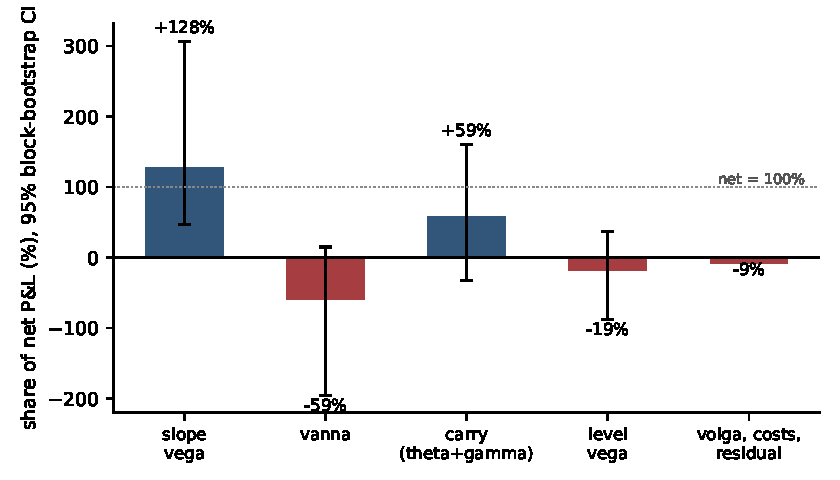
\includegraphics[width=0.75\textwidth]{fig_p4_attribution.pdf}
\caption{The attribution with bootstrap uncertainty. The slope engine's sign is essentially
certain; the shares of a five-year, one-instrument tape are, honestly, noisy.}
\label{fig:attr}\end{figure}

Two honest readings of Table~\ref{tab:attr}. First, the ordering and signs that the
propositions predict are what the data show, and the slope engine's positivity is
near-certain (99.7\% of draws). Second, the \emph{shares} are noisy---the vanna share's 95\%
interval marginally includes zero (negative in 94\% of draws). We emphasize that
Proposition~4's claim does not rest on the bucket bootstrap: the \emph{per-side} signs rest on
the per-leg analytic signs (Proposition~2) times the measured leverage covariance, and the
direction split of Table~\ref{tab:split} confirms both predicted signs, with the covariance
itself measured at $t = -19.2$ and $-7.1$---far
more precisely than a five-year P\&L share can be. The bootstrap honestly prices
what one instrument-half-decade of daily data can say about a decomposition's shares; it is
reported so that no reader mistakes an exact reconciliation for a precise attribution.
Cross-checks: wing Greeks were verified against vendor implied volatilities to 0.2--1.3\%,
and the decomposition's exactness (shares summing to 100.0\%) is an identity check run on
every build, not a rounding statement.

\section{The hedging bound, and forty-five failures}\label{sec:hedge}
The idealized counterfactual ``remove the vanna drag'' would lift the structure's performance
by the drag's share. Realizing it requires neutralizing $\Va_{\mathrm{net}}$ \emph{while
keeping} $\mathcal V_{\mathrm{net}} \approx 0$---two linear constraints. The two legs of the
risk reversal are spent (delta-match and skew direction), so a hedge needs \emph{two}
additional strikes $\{h_1, h_2\}$ solving
\[ \begin{pmatrix} \Va_{h_1} & \Va_{h_2} \\ \mathcal V_{h_1} & \mathcal V_{h_2} \end{pmatrix}
   \begin{pmatrix} n_{h_1} \\ n_{h_2} \end{pmatrix} =
   \begin{pmatrix} -\Va_{\mathrm{net}} \\ 0 \end{pmatrix}, \]
each crossing its half-spread at every rebalance. The achievable improvement is therefore
bounded by
\[ \Delta \;\propto\; \big|\mathbb E[(\mathrm V)]\big| \;-\;
   \textstyle\sum_j |n_{h_j}| \cdot \tfrac12 \mathrm{spread}_{h_j} \cdot (\text{rebalances}), \]
and the bound is an \emph{upper} bound in a further sense it ignores: the hedge strikes also
perturb the structure's carry and volga and drift between rebalances, so the comparison above
prices only the vanna-versus-spread component. In our data, forty-five realistic
implementations---five constructions (same-tenor 25-delta call, put, and call-plus-put joint
solve; cross-tenor call and call-plus-put) $\times$ three hedge ratios
$\{0.25, 0.5, 1.0\}$ $\times$ three rebalance cadences \{never, weekly, daily\}, every hedge
trade crossed at half-spread plus commission---all reduce net performance: the best variant
loses 0.15 of annualized Sharpe against the unhedged baseline and the worst loses 2.37
(Appendix~A, Table~\ref{tab:hedge45}). The Greek decomposition of the overlays shows why: at
the ratios that meaningfully offset the vanna bucket, the overlay either shorts the slope
engine itself (the joint-solve constructions are, at full ratio, the opposite risk reversal)
or pays recurring friction and carry exceeding the drag removed. The cheaper
response suggested by Proposition~4 is to condition \emph{exposure} on the spot--volatility
covariation regime rather than hedge the coupling; evaluating that lever is outside this
paper's scope, and we note that in our broader program every tested regime-conditioning
overlay has failed out-of-sample, so the prior is not favorable.

\section{Implications}
(1) \textbf{What the structure is}: a slope-vega skew-reversion engine on the cheap side and a
carry collector on the rich side, with a leverage-covariance transfer flowing from the
latter---not a vanna trade. (2) \textbf{Where the alpha is}:
the slope engine alone; it is orthogonal and stackable, while the carry crowds any
short-volatility book and should be budgeted as beta. (3) \textbf{Why the lore holds}:
volatility-normalization, path features, intraday clocks, and vanna hedges all fail for
reasons Proposition~3 and the hedging bound make structural rather than empirical.
(4) \textbf{What would change the economics}: only cheaper wings (the hedging bound loosens)
or a structural change in the leverage covariance (the toll shrinks)---both observable, neither
controllable.

\section{Limitations}
A note on what kind of contribution this is: the qualitative facts underlying Propositions~1
and~2---that delta-matching leaves the risk reversal nearly level-vega-neutral, and that its
wing vannas oppose in sign---are known to options practitioners and appear informally in the
trading literature \citep{sinclair}. What we claim is their formal statement, the
impossibility argument of Proposition~2 (stated with its tenor condition), the harvest
expression of Proposition~3 with its
observable companions, the identification of the vanna term as a direction-signed covariance
transfer with a
closed-form expectation, and an attribution that reconciles to a real tape. A reader who
regards formalisation of known practice as a modest contribution is not misreading the paper.
Beyond that: one underlying (SPY: American-style, dividend-paying; the derivations use European Greeks and
the empirical anchors absorb the difference); one wing delta studied in depth; 886 trades over
5.7 years, so the attribution shares carry the wide intervals of Table~\ref{tab:attr}, and the
direction split's side-net denominators are smaller still. The attribution basis is
sticky-strike, and the headline shares are coordinate statements---quantifiably so: the
sticky-strike slope innovation the attribution books loads on spot at $+0.48$ (Result~5),
while the \emph{fixed-delta} 10-delta risk-reversal change loads at $-0.89$ volatility points
per 1\% spot return with $R^2 = 0.38$---the two coordinate systems disagree even in the sign
of the spot coupling, because a down move drags fixed strikes toward the money along the skew
while steepening the fixed-delta smile. Roughly a third of the fixed-delta slope's variance is
spot-induced and would reclassify between the slope and vanna buckets under a smile-dynamics
basis. The direction-conditional \emph{signs} of Table~\ref{tab:split} are the
basis-robust content; a full re-attribution under a smile-dynamics basis is the natural next
exercise and is not performed here. The OU
model of the skew is a reduced form (its sufficiency is supported by corollary (ii) of
Proposition~3 rather than assumed); and the strategy-level orthogonality of Result~5 is
an empirical property of the studied sample, not a theorem.

\appendix
\section{The forty-five vanna-hedge variants}
\begin{table}[h]\centering\footnotesize\setlength{\tabcolsep}{4pt}
\begin{tabular}{llcccccc}\toprule
Constr. & Ratio & Rebal. & $\Delta$Sharpe & $\Delta$maxDD & Overlay P\&L & Overlay cost & Vanna offset \\
& & & vs.\ unhedged & (pp) & (\% of net) & (\% of net) & (\% of drag) \\ \midrule
ST-C & 0.25 & never & $-0.21$ & $-1$pp & $-17\%$ & $10\%$ & $+24\%$ \\
ST-C & 0.25 & weekly & $-0.45$ & $-10$pp & $-45\%$ & $26\%$ & $+14\%$ \\
ST-C & 0.25 & daily & $-0.69$ & $-12$pp & $-80\%$ & $69\%$ & $+23\%$ \\
ST-C & 0.50 & never & $-0.41$ & $-2$pp & $-33\%$ & $20\%$ & $+47\%$ \\
ST-C & 0.50 & weekly & $-0.67$ & $-12$pp & $-73\%$ & $46\%$ & $+34\%$ \\
ST-C & 0.50 & daily & $-1.03$ & $-21$pp & $-139\%$ & $111\%$ & $+46\%$ \\
ST-C & 1.00 & never & $-0.66$ & $-5$pp & $-67\%$ & $40\%$ & $+94\%$ \\
ST-C & 1.00 & weekly & $-0.90$ & $-16$pp & $-123\%$ & $79\%$ & $+75\%$ \\
ST-C & 1.00 & daily & $-1.30$ & $-28$pp & $-225\%$ & $170\%$ & $+91\%$ \\
ST-P & 0.25 & never & $-0.81$ & $-6$pp & $-98\%$ & $19\%$ & $+23\%$ \\
ST-P & 0.25 & weekly & $-0.95$ & $-6$pp & $-115\%$ & $35\%$ & $+27\%$ \\
ST-P & 0.25 & daily & $-1.18$ & $-19$pp & $-134\%$ & $97\%$ & $+31\%$ \\
ST-P & 0.50 & never & $-1.31$ & $-22$pp & $-196\%$ & $38\%$ & $+47\%$ \\
ST-P & 0.50 & weekly & $-1.44$ & $-28$pp & $-228\%$ & $65\%$ & $+54\%$ \\
ST-P & 0.50 & daily & $-1.52$ & $-32$pp & $-241\%$ & $162\%$ & $+62\%$ \\
ST-P & 1.00 & never & $-1.47$ & $-29$pp & $-392\%$ & $75\%$ & $+93\%$ \\
ST-P & 1.00 & weekly & $-1.54$ & $-32$pp & $-420\%$ & $119\%$ & $+106\%$ \\
ST-P & 1.00 & daily & $-1.63$ & $-35$pp & $-443\%$ & $248\%$ & $+122\%$ \\
ST-2 & 0.25 & never & $-0.25$ & $-2$pp & $-47\%$ & $13\%$ & $+25\%$ \\
ST-2 & 0.25 & weekly & $-0.17$ & $-2$pp & $-34\%$ & $14\%$ & $+26\%$ \\
ST-2 & 0.25 & daily & $-0.15$ & $-1$pp & $-26\%$ & $22\%$ & $+30\%$ \\
ST-2 & 0.50 & never & $-0.71$ & $-5$pp & $-94\%$ & $26\%$ & $+49\%$ \\
ST-2 & 0.50 & weekly & $-0.44$ & $-4$pp & $-68\%$ & $28\%$ & $+52\%$ \\
ST-2 & 0.50 & daily & $-0.34$ & $-2$pp & $-50\%$ & $41\%$ & $+60\%$ \\
ST-2 & 1.00 & never & $-2.34$ & $-54$pp & $-187\%$ & $53\%$ & $+99\%$ \\
ST-2 & 1.00 & weekly & $-1.33$ & $-27$pp & $-136\%$ & $57\%$ & $+104\%$ \\
ST-2 & 1.00 & daily & $-0.80$ & $-7$pp & $-98\%$ & $77\%$ & $+119\%$ \\
XT-C & 0.25 & never & $-0.22$ & $-1$pp & $-15\%$ & $10\%$ & $+24\%$ \\
XT-C & 0.25 & weekly & $-0.17$ & $-2$pp & $-7\%$ & $26\%$ & $+14\%$ \\
XT-C & 0.25 & daily & $-0.69$ & $-9$pp & $-76\%$ & $64\%$ & $+24\%$ \\
XT-C & 0.50 & never & $-0.43$ & $-2$pp & $-30\%$ & $21\%$ & $+49\%$ \\
XT-C & 0.50 & weekly & $-0.38$ & $-3$pp & $-22\%$ & $46\%$ & $+35\%$ \\
XT-C & 0.50 & daily & $-1.02$ & $-20$pp & $-125\%$ & $104\%$ & $+48\%$ \\
XT-C & 1.00 & never & $-0.68$ & $-5$pp & $-61\%$ & $41\%$ & $+98\%$ \\
XT-C & 1.00 & weekly & $-0.63$ & $-7$pp & $-49\%$ & $78\%$ & $+78\%$ \\
XT-C & 1.00 & daily & $-1.21$ & $-29$pp & $-187\%$ & $163\%$ & $+96\%$ \\
XT-2 & 0.25 & never & $-0.26$ & $-2$pp & $-46\%$ & $13\%$ & $+25\%$ \\
XT-2 & 0.25 & weekly & $-0.19$ & $-2$pp & $-35\%$ & $15\%$ & $+26\%$ \\
XT-2 & 0.25 & daily & $-0.23$ & $-2$pp & $-34\%$ & $27\%$ & $+31\%$ \\
XT-2 & 0.50 & never & $-0.75$ & $-4$pp & $-91\%$ & $27\%$ & $+51\%$ \\
XT-2 & 0.50 & weekly & $-0.50$ & $-4$pp & $-71\%$ & $31\%$ & $+53\%$ \\
XT-2 & 0.50 & daily & $-0.45$ & $-4$pp & $-60\%$ & $48\%$ & $+62\%$ \\
XT-2 & 1.00 & never & $-2.37$ & $-54$pp & $-183\%$ & $54\%$ & $+101\%$ \\
XT-2 & 1.00 & weekly & $-1.45$ & $-30$pp & $-142\%$ & $61\%$ & $+106\%$ \\
XT-2 & 1.00 & daily & $-0.94$ & $-9$pp & $-111\%$ & $86\%$ & $+124\%$ \\
\bottomrule\end{tabular}
\caption{All forty-five vanna-hedge implementations, each as a change against the identical
unhedged sleeve (Sharpe and maximum-drawdown deltas are scale-free; overlay P\&L and its
friction cost are shares of the sleeve's net, respecting the redaction). Constructions:
ST-C/ST-P = same-tenor 25-delta call/put sized to the stated ratio of position vanna; ST-2 =
same-tenor call-plus-put joint solve (overlay vega zero); XT = cross-tenor analogues. Every
hedge trade pays half-spread plus commission. No variant clears the pre-registered bar; the
best (ST-2, ratio 0.25, daily) still loses 0.15 of Sharpe.}
\label{tab:hedge45}\end{table}

\begin{thebibliography}{99}\small
\bibitem[Bakshi and Kapadia(2003)]{bakshi} Bakshi, G., Kapadia, N. (2003). Delta-hedged gains
and the negative market volatility risk premium. \emph{Review of Financial Studies} 16(2).
\bibitem[Bergomi(2016)]{bergomi} Bergomi, L. (2016). \emph{Stochastic Volatility Modeling}.
Chapman \& Hall/CRC.
\bibitem[Bollen and Whaley(2004)]{bw} Bollen, N., Whaley, R. (2004). Does net buying pressure
affect the shape of implied volatility functions? \emph{Journal of Finance} 59(2).
\bibitem[Carr and Wu(2009)]{carrwu} Carr, P., Wu, L. (2009). Variance risk premiums.
\emph{Review of Financial Studies} 22(3).
\bibitem[Castagna and Mercurio(2007)]{cm} Castagna, A., Mercurio, F. (2007). The vanna-volga
method for implied volatilities. \emph{Risk}, January.
\bibitem[Dennis and Mayhew(2002)]{dm} Dennis, P., Mayhew, S. (2002). Risk-neutral skewness:
evidence from stock options. \emph{Journal of Financial and Quantitative Analysis} 37(3).
\bibitem[Gatheral(2006)]{gatheral} Gatheral, J. (2006). \emph{The Volatility Surface}. Wiley.
\bibitem[G\^arleanu et al.(2009)]{gpp} G\^arleanu, N., Pedersen, L., Poteshman, A. (2009).
Demand-based option pricing. \emph{Review of Financial Studies} 22(10).
\bibitem[Mixon(2011)]{mixon} Mixon, S. (2011). What does implied volatility skew measure?
\emph{Journal of Derivatives} 18(4).
\bibitem[K\"unsch(1989)]{kunsch} K\"unsch, H. (1989). The jackknife and the bootstrap for
general stationary observations. \emph{Annals of Statistics} 17(3).
\bibitem[Sinclair(2013)]{sinclair} Sinclair, E. (2013). \emph{Volatility Trading}, 2nd ed.
Wiley, ch.~7.
\end{thebibliography}
\end{document}
